\clearpage
\section*{Appendix B: The mixed-effects cumulative logit model used for Experiment 2}
Data were analyzed using R \citep{RCT2014}, specifically with mixed-effects cumulative logit model using the \texttt{ordinal} package \citep{Christensen2015}.  For ordered response categories $1, 2, \dots, N$, a mixed-effects cumulative logit model specifies response probabilities for a given datum $i$ as a function of predictor variables as follows.  There are $N-1$ linear predictors, each of the following form:
%
\begin{align*}
  \eta_{ij} & = \alpha_j + \sum_{k} \beta_k x_{ik} + \sum_{k} b_k z_{ik} & j \in \{1, 2, \dots, N-1\}
\end{align*}
%
where the $\{x_{ik}\}$ and $\{z_{ik}\}$ are fixed- and random-effects predictors respectively,  the $\{\beta_k\}$ and $\{b_k\}$ are fixed- and random-effects regression parameters respectively, and $\alpha_i$ is a \textsc{threshold parameter} for the boundary between the $j$-th and $(j+1)$-th response categories.  (The threshold parameters play a role analogous to the intercept in an ordinary mixed logit model.)  The linear predictors are related to cumulative probabilities $\{\gamma_{ij}\}$ through the inverse logit function:
%
\begin{align*}
  \gamma_{ij} = P(Y_i \leq j) = \frac{e^{\eta_{ij}}}{1+e^{\eta_{ij}}}
\end{align*}
%
The probability of datum $i$ having response category $j$ is thus
%
\begin{align*}
  P(Y_i = j) =
  \begin{cases}
    \gamma_{i1} & j=1\\
    \gamma_{ij} - \gamma_{ij-1} & j \in \{2, \dots, N-1\}\\
1-\gamma_{ij-1} & j=N
  \end{cases}
\end{align*}
%
That is, the $\{\gamma_{ij}\}$ carve up the interval $[0,1]$ into a set of category response probabilities, as illustrated in Figure~\ref{fig:cumulative-logit-models}.  In mixed-effects cumulative logit models, the random-effects regression parameters are assumed to be drawn from some multivariate normal distribution, the covariance matrix of which is estimated jointly along with  the threshold parameters and fixed-effects regression parameters (here, via Laplace-approximated maximum likelihood).

\begin{figure}[ht!]
  \centering
  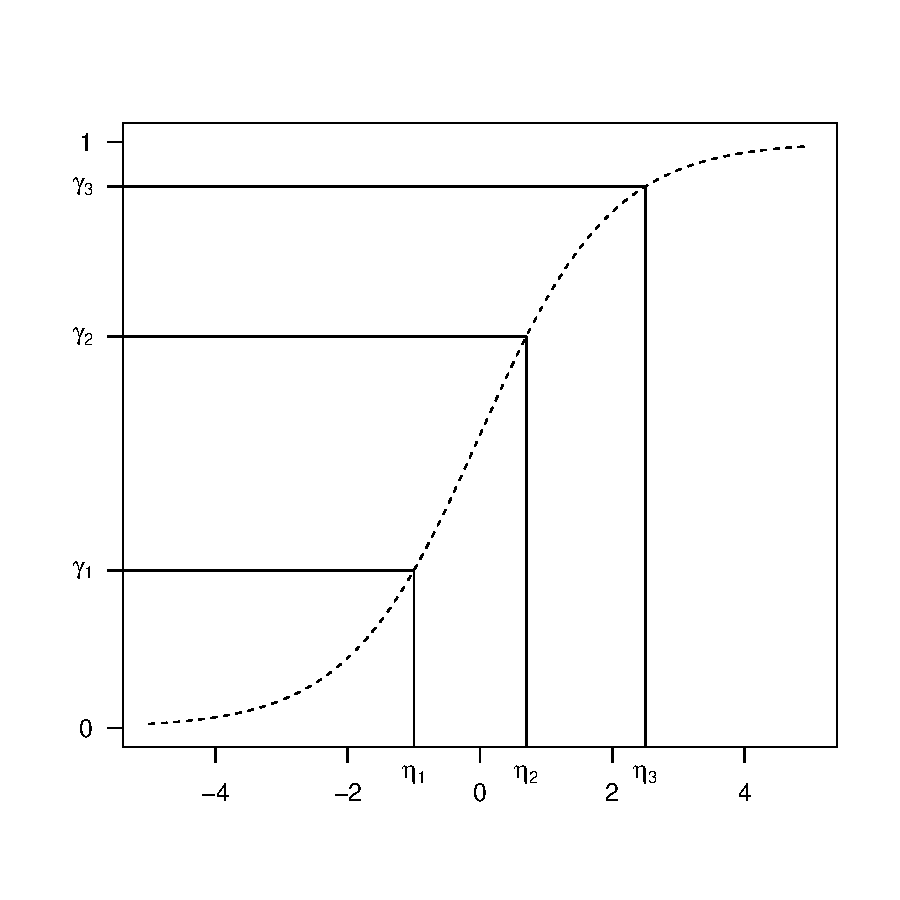
\includegraphics[width=.8\textwidth]{Figures/cumulative-logit-models}
  \caption{Cumulative logit models.  The $N-1$ linear predictors $\{\eta_j\}$ induce a set of $N$ multinomial response category probabilities through the inverse logit transform. }
  \label{fig:cumulative-logit-models}
\end{figure}